

\documentclass{article}
\usepackage{authblk}
\usepackage{setspace}
\usepackage[margin=1.25in]{geometry}
\usepackage{graphicx}
\usepackage{subcaption}
\usepackage{algorithm}       
\usepackage{algpseudocode}
\usepackage{amsmath}
\usepackage{booktabs}
\usepackage{float}
% \usepackage{subcaption}
% \usepackage{lineno}
% \linenumbers

% Set this if you want to limit how deep number of sections goes
% \setcounter{secnumdepth}{2}

%%%%%% Bibliography %%%%%%
% Replace "sample" in the \bibliography line at the bottom with the name of your .bib file.
\usepackage[numbers]{natbib}
\usepackage[colorlinks=true, linkcolor=black, citecolor=blue]{hyperref}
\usepackage{url}

%%%%%% Title %%%%%%
% Full titles can be a maximum of 200 characters, including spaces. 
% Title Format: Use title case, capitalizing the first letter of each word, except for certain small words, such as articles and short prepositions
\title{AI to Play the Card Game Oh Hell using Information Set Monte Carlo Tree Search (ISMCTS)}

%%%%%% Author %%%%%%
% Put your full names as you want it to appear here
\author{Owen Suelflow}

%%%%%% Affiliations %%%%%%
\affil{Macalester College}


%%%%%% Date %%%%%%
% Date is optional
\date{}

%%%%%% Spacing %%%%%%
% Use paragraph spacing of 1.5 or 2 (for double spacing, use command \doublespacing)
\onehalfspacing

\begin{document}

\maketitle

%%%%%% Abstract %%%%%%
{\singlespacing
\begin{abstract}
    We present an AI player to play the card game Oh Hell using Information Set Monte Carlo Tree Search (ISMCTS).
    The game is first introduced and similar approaches to this problem are discussed. Then, we detail our bidding algorithm as well as the methods we used to create the playing engine for our AI. We then produce
    simulated experiments to analyze the strength of the AI player, what impacts its skill, and how it plays.
\end{abstract}}

%%%%%% Main Text %%%%%%

\section{Introduction}
\label{section:Introduction}
In this paper, we investigate the aptitude of Information Set Monte Carlo Tree Search in playing the popular card game Oh Hell (also known as Nomination Whist and Up and Down the River.)
According to a YouGov poll in 2023, 29\% of adults in the United States reported that they played in-person card games often, and 28\% reported playing online card games. Given the popularity of card games, and
especially given the strong online card game presence, having a robust AI model to play these card games against human players is an important problem. 

Oh Hell is a trick-taking card game that uses a standard 52 card deck and can be played by 2-5 players.
A \textit{trick taking} game consists of some number of tricks, and for each trick, one player leads a card, and the other players must follow suit by playing a card from their hand of the same suit if possible.
They may play any card from their hand if they do not have a card of the suit that was lead. Play starts with the player who won the previous trick (or at the beginning of the game, the player to the left of the dealer), and goes clockwise. 
The winner of the trick is the player who played the highest card of the suit that was lead if no trumps were played, or the highest trump card if any trumps were played. 
A \textit{trump} card is a card whose suit is the trump suit, and in Oh Hell, the trump suit is determined at the beginning of a game by flipping over the top card in the deck.
Trump cards always beat any non-trump suited card.

The goal of each round is to win a certain number of tricks. At the beginning of each round, players go around, starting with the player to the left of the dealer, and \textit{bid} how many tricks they think they will win.
Then, play begins, and continues until all cards have been played. Players earn a score of 10 points plus the number of tricks they bid if they win the exact number of tricks bid, or 0 points if they don't earn their bid.
A \textit{game} consists of some number of rounds -- typically, play begins with a round of 10 tricks, then a round of 9 tricks, all the way down to 1 trick, and then rounds of 2, then 3, and so on back up to 10 tricks. 
The winner of the game is the player who has the most points accrued at the end of the game.

Building an AI to play card games like Oh Hell is challenging because card games are usually \textit{imperfect information} games. 
In a perfect information game like Chess and Go, all information in a given state is known to each player. Both of these games were famous problems for scientists to try and build algorithms to play them -- an early implementation of a Go AI player can be found in \citet{van2004ai}.
For trick-taking games like Oh Hell, game companies have used Information Set Monte Carlo Tree Search as the playing engine for their AI. This was first introduced by \citet{cowling2012information}, and used in their game company AI Factory for the popular card game Spades. Given Spades is quite similar to Oh Hell, ISMCTS makes sense as the method of choice for our work.

The rest of the paper is organized as follows: \textbf{Section~\ref{section:Background}} provides an overview of the work done in this area, mainly focusing on the work done by AI Factory, and \textbf{Section~\ref{section:Methodology}} defines our bidding algorithm, ISMCTS, and our method of determinization, particle filtering. 
Then in \textbf{Section~\ref{section:Analysis}}, we test our implementation in various experiments, showcasing its strength and the parameters that impact it, as well as analyzing how it plays. 
Finally in \textbf{Section~\ref{section:FutureWork}}, we highlight areas of future growth, and conclude by recapping our work in \textbf{Section~\ref{section:Conclusion}}.
 
\section{Background}
\label{section:Background}
Monte-Carlo Tree Search was first introduced as a general search framework by \citet{coulom2006mcts}, with later theoretical refinement through the UCT algorithm of \citet{kocsis2006uct}. More detail about early MCTS methods can be found in the oft-cited survey paper of \cite{browne2012survey}. 
From the standard MCTS approach, work has been done by \citet{cowling2012information} to develop ISMCTS, which works well specifically in games with imperfect information. A big challenge in imperfect information games is trying to model the information unknown to the player. 
When applying MCTS to trick taking games like Oh Hell, Hearts, and Spades, cards are dealt randomly to the other players so as to create a perfect information game, with simulation commencing afterwards. 
\citet{AIFactory2013}, \citep{winands2017magic} used ISMCTS in their mobile card game app for their AI player in Spades. They detail the algorithm and give a simple Python implementation by \citet{Cowling2013} that we use in our Oh Hell AI player. Further discussion of ISMCTS can be found in Section~\ref{subsection:ISMCTS}.
AI Factory also details their methodology for the determinization step in the ISMCTS algorithm in their Spades mobile game in \citep{rollason2018figuring} and \citep{rollason2019bidding_inferences}.
They employ probability tables, with the goal of determining the probability that each player holds a given card from the perspective of each of the players. They incorporate each player's bid, cards that are played during the run of play, and various heuristics developed based off of different playing strategies that mimic human thinking.

Another approach to making inferences during the determinization step of ISMCTS is shown in \citet{rebstock2019policy}. The team from the University of Alberta developed a Policy Based Inference using player modelling to assign a probability to each state that it was the true state. They used data from an online card game from real players to deduce playing strategy and to build a deep neural network to try to give a probability distribution of each possible adjacent state given the current game state.
While this approach wasn't possible for this project, the general idea of trying to emulate human thinking in the implementation of inferences is a solid one. In this paper, our method of choice is Particle Filtering. 
More detail can be found in \citep{cs188_particle_filtering}, and we give a brief overview of the method and our implementation in Section~\ref{subsection:ParticleFiltering}.

Finally, before the card playing commences, each player must bid how many tricks they think they will win. \citet{cohensius2019bidding} discusses a bidding algorthm implemented for Spades. 
The authors employ a metaheuristic that combines a rules-based bidding approach with a logistic regression model that trained on bidding data from over 2 million online Spades games. They use the logistic regression model to correct for anything the rules-based model missed. The rules-based approach utilized four main ways of winning a trick: off-suit high card, trump high card, trumping in, and extra trumps. We use a similar approach in this paper, with further discussion in Section~\ref{subsection:Bidding}.

\section{Methodology}
\label{section:Methodology}
In this section, we describe our implementation of our Oh Hell AI player. Oh Hell is naturally a two stage game -- the bidding round, and the playing round. As such, we deploy a separate algorithm for each of the stages. Section~\ref{subsection:Bidding} outlines our bidding algorithm, including discussion about different heuristics we employ as well as some Monte Carlo simulations used to generate probabilites relevant to bidding.
Section~\ref{subsection:ISMCTS} explains how the ISMCTS algorithm works, and Section~\ref{subsection:ParticleFiltering} unfolds how we determinize at each step of the ISMCTS algorithm.
\subsection{Bidding}
\label{subsection:Bidding}
In the first stage of Oh Hell, each player bid how many tricks they think they will, starting with the player to the left of the dealer. Players may bid zero tricks or may bid up to a maximum of the number of tricks in the round. 
The final player to bid, the dealer, cannot bid an amount of tricks that will make the sum of each player's bid equal to the number of tricks in the round. This ensures that one player must lose, hence the name "Oh, Hell".
The goal of our bidding algorithm is to use the player's hand, the bids of their opponents (if any), and the position in which they bid to determine the expected number of tricks they will win. 
First, we run through the special case of only having 1 trick, which deserves its own section as we can have much higher confidence in what the correct bid should be than in rounds with more than 1 trick. Next, we explain the three main ways that our algorithm assigns a non-zero probability of winning a trick with a given card. Then, we describe how we adjust the predicted bid based on what other players have bid and the bidding position of the player.
\subsubsection{Bidding With Only One Trick}
At this stage of the game, each player only has one card and so they can only play that card. Bidding is reduced to game of probability, impacted by two things: whether or not the player is bidding first, and if they hold a trump card or not. 
In Table~\ref{tab:oneTrickProbs}, we see the probability of winning the trick given the player's card and bidding position. There are a few scenarios to consider beyond just using the table.
First, if the player is bidding last, they are forced to bid 0 if nobody has bid, 1 if one player has bid, and in the very rare case in which more than one player has bid, the player should almost always bid 0 unless they have a very high trump card with rank greater than a Jack. 
Next, if the player is not leading and they have an off suit, they should bid 0. If they are not leading but have a trump card, and nobody has bid, they should bid. If someone has bid, it becomes a bit more complex and the player should only bid if they have a good enough trump card. Finally, if the player is the one leading, they can solely follow the probability table to decide if they should bid or not. If their situation has a greater than 50\% chance of winning, they should bid.
We also note that the last 3 columns of the side suit table are identical. This is because it doesn't matter what position we play if we aren't leading. With the trump suit, they're all identical, as again position of play does not matter -- everyone must play their card.
\begin{table}[h]
\centering
\caption{Tables denoting the probability of winning the final trick in a 4 player game given the player's bidding position (P1, P2, P3, or P4), the rank of their card, and trump (right table) or off suit (left table)}
\label{tab:oneTrickProbs}
\begin{minipage}{0.48\textwidth}
\centering
\begin{tabular}{r|cccc}
\hline
Rank & P1 & P2 & P3 & P4 \\
\hline
2  & 0.1323 & 0.0000 & 0.0000 & 0.0000 \\
3  & 0.1466 & 0.0057 & 0.0059 & 0.0056 \\
4  & 0.1668 & 0.0114 & 0.0118 & 0.0122 \\
5  & 0.1837 & 0.0197 & 0.0205 & 0.0192 \\
6  & 0.2066 & 0.0277 & 0.0272 & 0.0272 \\
7  & 0.2255 & 0.0371 & 0.0365 & 0.0373 \\
8  & 0.2512 & 0.0479 & 0.0468 & 0.0474 \\
9  & 0.2774 & 0.0606 & 0.0584 & 0.0587 \\
10 & 0.3041 & 0.0718 & 0.0714 & 0.0721 \\
11 & 0.3363 & 0.0877 & 0.0848 & 0.0868 \\
12 & 0.3627 & 0.0996 & 0.1000 & 0.1016 \\
13 & 0.3962 & 0.1176 & 0.1194 & 0.1171 \\
14 & 0.4294 & 0.1343 & 0.1344 & 0.1358 \\
\hline
\end{tabular}
\end{minipage}
\hfill
\begin{minipage}{0.48\textwidth}
\centering
\begin{tabular}{r|cccc}
\hline
Rank & P1 & P2 & P3 & P4 \\
\hline
2  & 0.4644 & 0.4654 & 0.4645 & 0.4651 \\
3  & 0.4997 & 0.4995 & 0.4990 & 0.4989 \\
4  & 0.5387 & 0.5347 & 0.5318 & 0.5370 \\
5  & 0.5754 & 0.5807 & 0.5829 & 0.5728 \\
6  & 0.6140 & 0.6180 & 0.6160 & 0.6175 \\
7  & 0.6571 & 0.6572 & 0.6607 & 0.6589 \\
8  & 0.6999 & 0.6985 & 0.7035 & 0.6973 \\
9  & 0.7480 & 0.7416 & 0.7513 & 0.7425 \\
10 & 0.7883 & 0.7864 & 0.7927 & 0.7882 \\
11 & 0.8384 & 0.8444 & 0.8380 & 0.8433 \\
12 & 0.8881 & 0.8881 & 0.8895 & 0.8913 \\
13 & 0.9450 & 0.9456 & 0.9441 & 0.9446 \\
14 & 1.0000 & 1.0000 & 1.0000 & 1.0000 \\
\hline
\end{tabular}
\end{minipage}
\end{table}

\subsubsection{High Card Off-Suit}
\label{subsubsection:highOff}
The simplest way to win a trick is by playing an off suit (non-trump suit) high card. For example if the trump suit is clubs and a player leads the ace of hearts, and all other players have a heart, then that player will win the trick. However, in order to guarentee that the player can win the trick with the high card, all the other players must have at least one card of the suit and cannot have a higher card. 
If this assumption were false, then there is a chance that another player could play a trump card or a higher card of the suit. We assume that, for each off suit, the first trick won in this fashion is won by the ace, and then the king, and so on. This is a strong assumption, but makes the probabilities easier to work with. In a game like Spades, where all 52 cards are dealt, we know for sure that all the high cards are in play. 
But in Oh Hell, not all cards are dealt. We define the probability of winning a trick in this fashion with a given off suit high card as follows, letting $n_p$ be the number of players in the game, $n_t$ be the number of tricks in the round, $n_{cp}$ be the number of cards with \textit{card's} suit, and $n_{op}$ be the minimum number of cards in \textit{card's} suit in each of the opponent's hands:
$$\Pr(\text{winTrick}|\textit{card}) = \Pr(n_{op} \geq (15-\textit{cardRank})|n_p,n_t,n_{cp})$$
In order to calculate these probabilities, we performed one million Monte Carlo simulations for each possible number of tricks in a round (1-10). Then, during the bidding process, we can easily look up probabilites as needed using the relevant probability table loaded up for the specific game parameters (number of tricks, number of players). 
An example probability table for a 10 trick, 4 person game is shown in Table\ref{tab:offSuitProbs}.

\begin{table}
\centering
\caption{Probability table for a 10 trick, 4 person game. Value in [$i$][$j$] gives the probability that, given the player has $i$ cards in an off suit, each opponent has at least $j$ cards in that suit.}
\label{tab:offSuitProbs}
\begin{tabular}{rrrrrr}
 & 0 & 1 & 2 & 3 & 4 \\
\midrule
0 & 1.0000 & 0.9656 & 0.7351 & 0.2431 & 0.0075 \\
1 & 1.0000 & 0.9469 & 0.6424 & 0.1435 & 0.0011 \\
2 & 1.0000 & 0.9201 & 0.5334 & 0.0702 & N/A \\
3 & 1.0000 & 0.8830 & 0.4136 & 0.0255 & N/A \\
4 & 1.0000 & 0.8300 & 0.2863 & 0.0051 & N/A \\
5 & 1.0000 & 0.7593 & 0.1687 & N/A & N/A \\
6 & 1.0000 & 0.6678 & 0.0760 & N/A & N/A \\
7 & 1.0000 & 0.5452 & 0.0205 & N/A & N/A \\
8 & 1.0000 & 0.4107 & N/A & N/A & N/A \\
\bottomrule
\end{tabular}
\end{table}
\subsubsection{High Card Trump Suit}
\label{subsubsection:highTrump}
The second way we can win is winning with a high trump card. If the player has a trump card with a rank of at least 10, we give that card an expected tricks value of one, given the extreme likelihood they will be able to win a trick with that card. For middling trump cards (6-9, generally), this can sometimes underpredict them, especially in games with few tricks, as the probability of any opponent having higher trumps gets lower. However, this is corrected later through some basic heuristics to ensure the trump bid is reasonable.
\subsubsection{Trumping In}
\label{subsubsection:trumpingIn}
The final way to win a trick in Oh Hell is by trumping in. This is a move that occurs when the player does not have a card in the off suit that was lead, and so is allowed to play any card they would like. Often this is a good chance to play a trump card if the player needs to win more tricks, as other players must follow suit if they are able while the trump card beats anything they play if they don't also trump in. 
We find the probability of winning a trick with a trump card by trumping in in a similar fashion to Section~\ref{subsubsection:highOff}:
$$\Pr(\text{trumpingIn}|\textit{card}) = \Pr(n_{op} \geq (1+n_{cp})|n_p,n_t,n_{cp})$$
Refer to Table~\ref{tab:offSuitProbs} as an example for exact probabilities for a 10 trick, 4 person game. If the player has one club and trump is diamonds, the probability that they can trump in on clubs is 0.6424. This is the probability that, in a 10 trick, 4 player game, all the other players have at least two clubs, and since the player only has one club, if clubs are lead again, they can play a trump and guarentee a win. This assumes that no clubs will be played in other tricks by other players.
\subsubsection{Adjusting For Other Players' Bids}
\label{subsubsection:adjOtherPlayers}
Finally, we must adjust the predicted bid to account for what the other players have bid, as well as when we are bidding. If the player is bidding first, no adjustment is needed as there is no other prior bidding information to go off of.
Otherwise, we use the following formula to adjust the player's bid, where $n_b$ is the number of bids made in the round and $p \in P$ represents for each player:
$$\text{newBid} = \text{predBid} - \frac{\sum_{p \in P}\text{Bid}_p - n_b\times\frac{n_t}{n_p}}{n_p-n_b}$$
Effectively, we check to see how far from the average bid $(n_t/n_p)$ the total bids are, and adjust based on that. Additionally, through empirical tests we needed to add an extra multiplier to increase the predicted bid as the player was systematically underbidding.
For games with 3 or more players, the player's bid is increased by a factor of 1.3, and for games with two players, the player's bid is increased by a factor of 1.13. Basic heuristics are then used at the end as a sanity check to make sure the player is not making an extremely poor bid. For example, a check is done to make sure the player is bidding at least one if they have a jack of trump or higher. Next, the player's bid is increased by one if they are deemed "aggressive", or decreased by one if they are deemed "passive". Finally, we deal with the case where the player is the last to bid and thus cannot bid a number of tricks that brings the total bids equal to the number of tricks. A full description of the bidding algorithm is shown in Algorithm~\ref{alg:bidding}.

\begin{algorithm}[H]
    \caption{Bidding Algorithm}
    \label{alg:bidding}
    \begin{algorithmic}[1]
        \State \textbf{function} Bid(player)
        \State expectedBid $\gets 0$
        \If{tricksInRound = 1}
            \If{last player to bid}
                \State Adjust bid to avoid total bids = tricksInRound
            \Else
                \State Use one trick probability table
                \If{high trump card and previous bids exist}
                    \State Possibly increment bid to 1
                \EndIf
            \EndIf
        \Else
            \State Count cards per suit, mark trump suit
            \For{each off-trump suit}
                \For{each card in suit}
                    \State Compute expected trick probability
                    \State expectedBid += max(probabilities)
                \EndFor
            \EndFor
            \State trumpBids $\gets$ 0
            \For{each card in trump suit}
                \State Compute expected trick probability
                \State trumpBids += max(probabilities)
            \EndFor
            \State predBid $\gets$ expectedBid + trumpBids
            \State Adjust predBid based on:
            \State \quad player position in bidding order
            \State \quad number of players
            \State \quad bidStyle (aggressive/passive)
        \EndIf
        \State bids[player] $\gets$ round(predBid)
    \end{algorithmic}
\end{algorithm}

\subsection{Information Set Monte Carlo Tree Search}
\label{subsection:ISMCTS}
Now that the AI player can bid properly, we must turn our attention to the trick-playing stage of the game. Here, we give a brief overview of our implementation of ISMCTS, following the work of \citet{cowling2012information} and code in \citep{Cowling2013}.
First, we introduce Monte Carlo Tree Search, the very similar algorithm that precluded ISMCTS. There are four steps in each iteration of MCTS, as shown in Figure~\ref{fig:mcts}.
\begin{enumerate}
    \item \textbf{Selection}: To begin, select a child state of the root state according to a multi-armed bandit algorithm. We use UCB1, which is used in \citep{cowling2012information} and most other MCTS applications. Then continue to choose children of each successive node until a node with untried moves is reached. The UCB1 algorithm is a way to balance exploitation (choosing a highly visited node) vs. exploration (choosing a relatively unexplored node).
    $$\text{UCB1(\textbf{Parent})} = \text{argmax}_{\text{child}\in \textbf{Parent}}\left(\frac{\text{totalReward}_{child}}{\text{numVisits}_{child}} + c\sqrt{\frac{\log(\text{numVisits}_{\textbf{Parent}})}{\text{numVisits}_{child}}}\right)$$
    The first term is just the average reward, representing the exploitation term. The second term can be thought of as the relative amount of exploration of the child node. The parameter $c$ controls this tradeoff. \citet{cowling2012information} used $c=0.7$, which seems to be the common choice when rewards are between 0 and 1. Even though the scoring for Oh Hell is not between 0 and 1 (0 or 10 + number of tricks won), we can normalize the score to be between 0 and 1.
    \item \textbf{Expansion}: Randomly choose one of the unexplored moves and it to the tree.
    \item \textbf{Simulation}: Starting at the state corresponding to the expanded node, apply random moves until the end of the game is reached.
    \item \textbf{Backpropogation}: Update the win and visit counters for each node that was just visited from the expanded node, including the note itself.
\end{enumerate}
We note that our "win" value must be between 0 and 1 for the UCB1 algorithm to work properly. As such, we have two ways of quantifying a player's score at the end of the game. At the beginning of the game, the AI player chooses which of the two scores they will use. If they choose to only use their own score, we have
$$\text{Win}(terminalState) =\left\{ \begin{array}{cc}  1 & \text{If player has earned their bid in the terminal state } \\ 0 & \text{Otherwise}\end{array}\right.$$
However, incorporating the scores of the other players might be more useful. Oh Hell is typically played with many rounds, with players accruing points over time. So, it is beneficial to not only try to score points, but limit the scores of the other players.
This is especially true if the AI player has reached a point in the game where they have won more tricks than they bid. At this point, it is impossible for it to earn points, so if it only cared about its own score, it would just play random moves until the end of the round. It could instead try to win lots of tricks in order to mess up its opponents and have them earn 0 points as well.
We calculate its win reward in this scoring environment as follows:
$$\text{Win}(terminalState) = \textbf{Normalize}(\text{Score}-\text{avg}(\text{Other Players' Scores}))$$
Now, we briefly introduce ISMCTS. It is very similar to MCTS, just with an added step in the beginning.
\begin{enumerate}
    \item \textbf{Determinization}: Randomize information hidden from the player in the root state using Particle Filtering by sampling from the player's particle set.
    \item \textbf{Selection}: Same as MCTS, but child nodes must be compatible with the determinized state
    \item \textbf{Expansion}: Same as MCTS
    \item \textbf{Simulation}: Same as MCTS
    \item \textbf{Backpropogation}: Same as MCTS
\end{enumerate}
The determinization step is what will require the most work, and what most impacts the performance of ISMCTS beyond running the algorithm for more iterations. In the next section, we define our method for determinizing, particle filtering.
\begin{figure}[htbp]
\centering
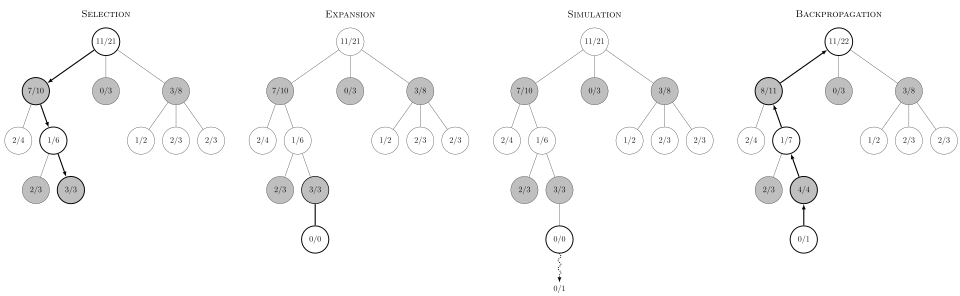
\includegraphics[width=\linewidth]{MCTS-steps.svg.png}
\caption{Illustration of the four phases of Monte Carlo Tree Search.
Source: Wikipedia~\cite{wiki:mcts}.}
\label{fig:mcts}
\end{figure}


\subsection{Particle Filtering}
\label{subsection:ParticleFiltering}
Particle filtering (also known as Sequential Monte Carlo) is a bayesian technique used for state space estimation in non-linear state space models. In our Oh Hell AI player, particle filtering comes into play during the determinization phase of ISMCTS. 
In PF, the player has a set of particles and an associated set of weights where each weight represents the likelihood of corresponding particle representing the true information. In Oh Hell, each particle contains cards assigned to each of the opposing players.
At the beginning of the game, the AI player initializes its set of particles, which we denote by $\phi$, and initializes its set of weights, denoted by $\omega$. Each weight $\omega_i$ gets set to $\omega_i=\frac{1}{|\phi|}$. The process for maintaining the AI player's particle set is as follows:
\begin{algorithm}[H]
    \caption{Updating Particles}
    \label{alg:particleFiltering}
    \begin{algorithmic}[1]
        \State \textbf{function} updateParticles(move)
        \For{every particle}
            \State Check if move in particle and update weight accordingly
            \State Check if move did not follow suit and update weight accordingly
            \State Make inferences and update weight
        \EndFor
        \If{Every particle has weight 0}
            \State Regenerate Particles
            \State Reset weights to uniform
        \EndIf
        \If{$\text{ESS} < 0.3\times|\phi|$}
            \State Resample Particles
            \State Reset weights to uniform
        \Else
            \State Normalize weights
        \EndIf
    \end{algorithmic}
\end{algorithm}

The idea is that we have some prior belief about what the distribution of potential hands for the opposing players looks like, and then we update these beliefs as we get new information. This new information is almost predominantly from an opponent playing a card. 
The only exception is at the beginning of the game, as the AI player can glean information about the strength of their opponent's hand by what they bid. 
To update the particles when a move is played, we first find all particles that are no longer valid. This could occur in a number of ways: The card that was played wasn't in that player's hand, the card was in no one's hand, or, in the case of the card not following suit, that player's hand contained cards of the leading suit.
This usually leads to many particles $(>50\%)$ becoming invalid. 

To help mitigate the loss of so many particles, we relax the need for the \textit{exact} card to be in the current player's hand. For example, if the current player played the 4 of clubs, and one of the particles for the AI player has the current player holding a 5 of clubs, we treat those cards as the same. 
Effectively, having a card that is one or two ranks off from the actual card played doesn't change the strength of the player's hand, so we don't need to set that weight to zero. 

Then, we make inferences. This is an expensive part of the algorithm, and as such we only employ one heuristic. For each particle with non-zero weight, we run our bidding algorithm on each of the players hands within the particle. Then we update the \textit{logweight} based on how well the bids of the particle match up with the actual number of tricks each of the players has to win.
This is done in logspace to avoid potential underflow errors.
$$\log(\omega_i) = \log(\omega_i) - \lambda\sum_{p \in \phi_i}\left|\text{predBid}_p-\text{tricksNeeded}_p\right|$$

Here, $\omega_i$ represents the weight of the $i$th particle, and $p \in \phi_i$ represents going through each player's hand in the $i$th particle. The $\lambda$ parameter controls how severely particles that have a poor reflection of the true strengths of each players hand. If $\lambda = 2$, then for every one trick error between the predicted tricks won versus the actual tricks needed to win, the particle weight is two times less likely compared to a particle that exactly matches the trickes needed.
We've experimentally chosen $\lambda$ to be 1.3. This heuristic is performed at the beginning of the game after initializing particles, and after any time the particles get regenerated.

Next, if after updating particles, none of them have nonzero weight, we must regenerate. To regenerate, we follow a similar process to initializing the particles in the beginning of the game. This time, there is more information that we know, either from players playing cards or from players being void in a suit. Each new particle must be valid with respect to our previous information.
Once we have a new set of particles, we run our bidding heuristic to update their weights.

Finally, if we did not regenerate, we check to see if particles need to be resampled if too many of them have zero or near zero weight. We can quantify this using Effective Sample Size (ESS).
$$\text{ESS} = \frac{1}{\sum_{i=1}^{|\omega|}\omega_i^2}$$
ESS is equal to $1/|\omega|$ if each particle has uniform weight. If $ESS < 0.3|\omega|$, then we resample using systematic resampling. This technique is similar to multinomal sampling, where we just sample from the distribution of particles without replacement, but with small tweaks that reduce the variance.
\begin{algorithm}[H]
    \caption{Systematic Resampling}
    \label{alg:sysResampling}
    \begin{algorithmic}[1]
        \State \textbf{function} systematicResample()
        \State $n = |\omega|$
        \State Normalize Weights
        \State $C_j = \sum_{k=1}^j \omega_k \ \forall j \in {1, 2, \dots, n}$
        \State Let $\mu ~ \text{Uniform(0,1/n)}$
        \State Create $n$ equally spaced points $\alpha_i = \mu + \frac{i-1}{n} \ \forall i \in {1, 2, \dots, n}$
        \For{each $\alpha_i$}
        \State Find smallest $j$ such that $C_j < \alpha_i$
        \State Add particle $\phi_j$ to new set of particles
        \EndFor
    \end{algorithmic}
\end{algorithm}

After resampling, we are done and we return to the game for the next player's move. Then, we do it all over again.

\section{Analysis}
\label{section:Analysis}
Finally, it is time to play the game. How does our AI player perform? Unfortunately, unlike in \citep{Cowling2013}, \citep{rebstock2019policy}, and \citep{cohensius2019bidding}, we don't have access to an online game in which we can deploy our model and get massive amounts of data of games against real players.
So, we must design our own experiments to try and analyze how the AI plays, in addition to playing it ourselves. We orchestrate 10s of thousands of simulated games with various parameters and various number of AI players. This way, we can analyze how well the AI plays, what parameters impact the quality of its play, and how it plays.

Shown in Figure~\ref{fig:mcparts} is the win percentage for the AI player, defined as if they won their bid in tricks or not, across different numbers of ISMCTS iterations and numbers of particles. Each permutation had close to 200 games simulated, with the AI player playing against 3 players playing random (legal) moves. The plot shows a general trend that more particles and more iterations leads to a higher win percentage. Given the smaller sample size for each permutation, there is some noise in the data, causing the trend to not behave exactly as we'd expect.
It's also interesting to note that the win percentages are relatively low. This is due to the fact that our AI player is making inferences based off of how a rational player would play during the game. But since each opponent is making random moves (i.e. acting irrationally), some of those heuristics fall flat. The game becomes more of a game of chance than strategy at that point.
\begin{figure}[H]
\centering
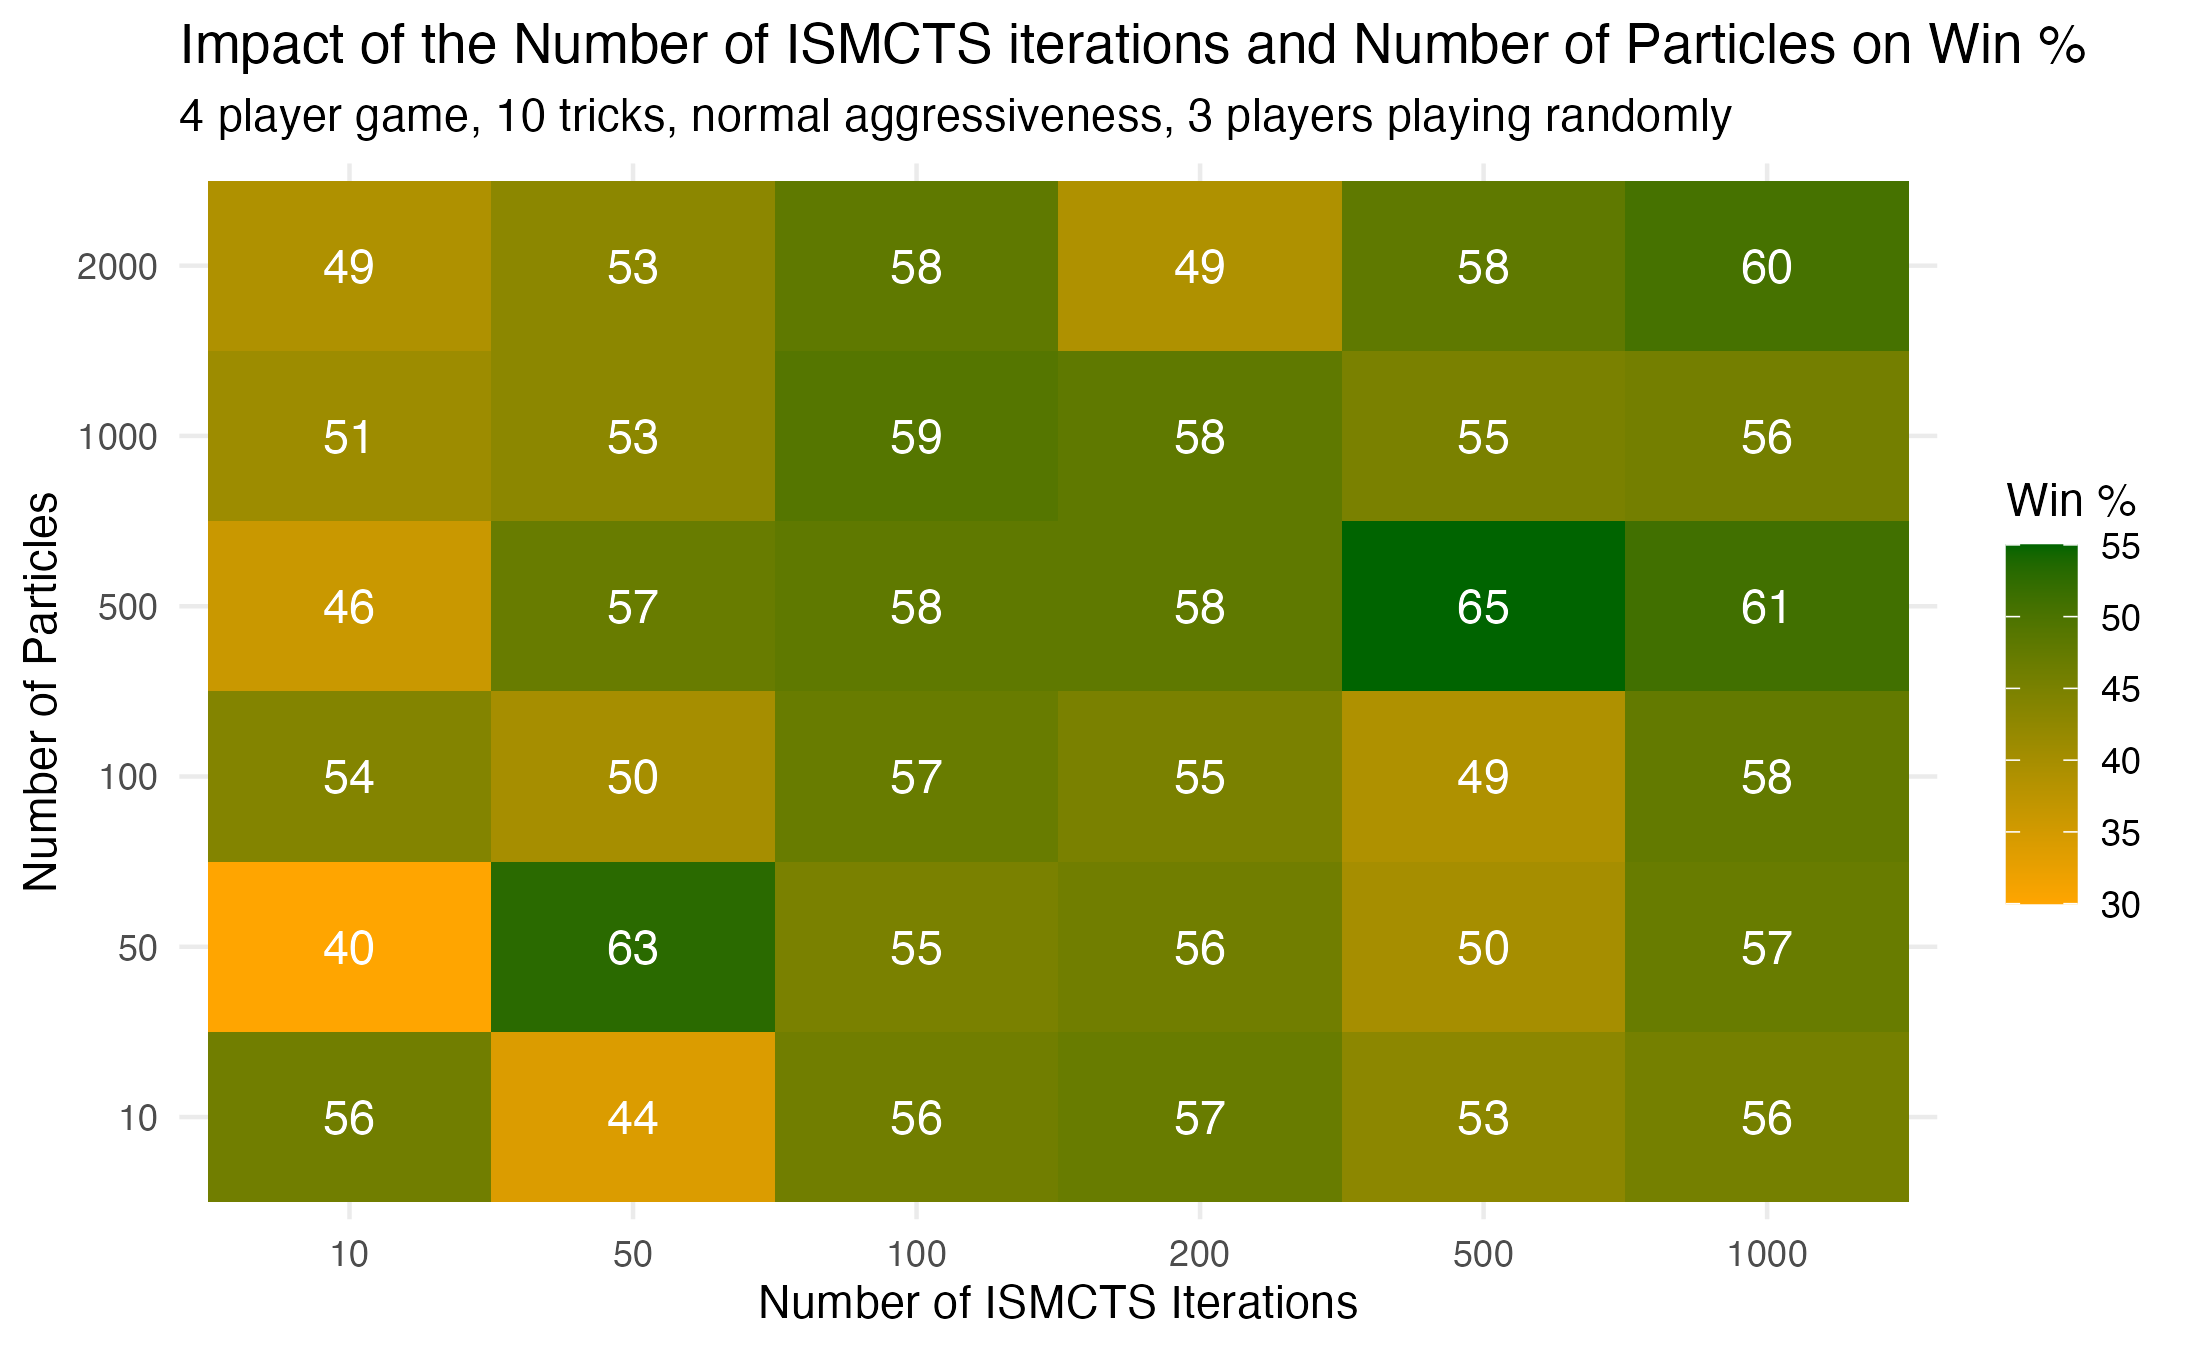
\includegraphics[width=\linewidth]{mcvsparticles.png}
\caption{Comparing performance of AI player for different number of particles and ISMCTS iterations}
\label{fig:mcparts}
\end{figure}


In our next experiment, we different values of $\lambda$, the parameter that impacts how drastically particles are punished if their overall perceived bid strength doesn't match up with the true amount of tricks the other players still need to win. We test 7 different $\lambda$ values, along with varying amounts of particles. The results are shown in Figure~\ref{fig:partslambda}.
It seems that the choice of $\lambda$ does not have a huge impact on win percentage, though higher values of $\lambda$ generally seem to do worse. This analysis comfirmed that our choice of $\lambda = 1.3$ is a reasonable choice. With higher values, the AI player places too much emphasis on particles whose hand strength matches reality, which prevents the player from sampling from a more diverse set of hands and effectively is overfitting the model of the opposing players' hands.

\begin{figure}[H]
\centering
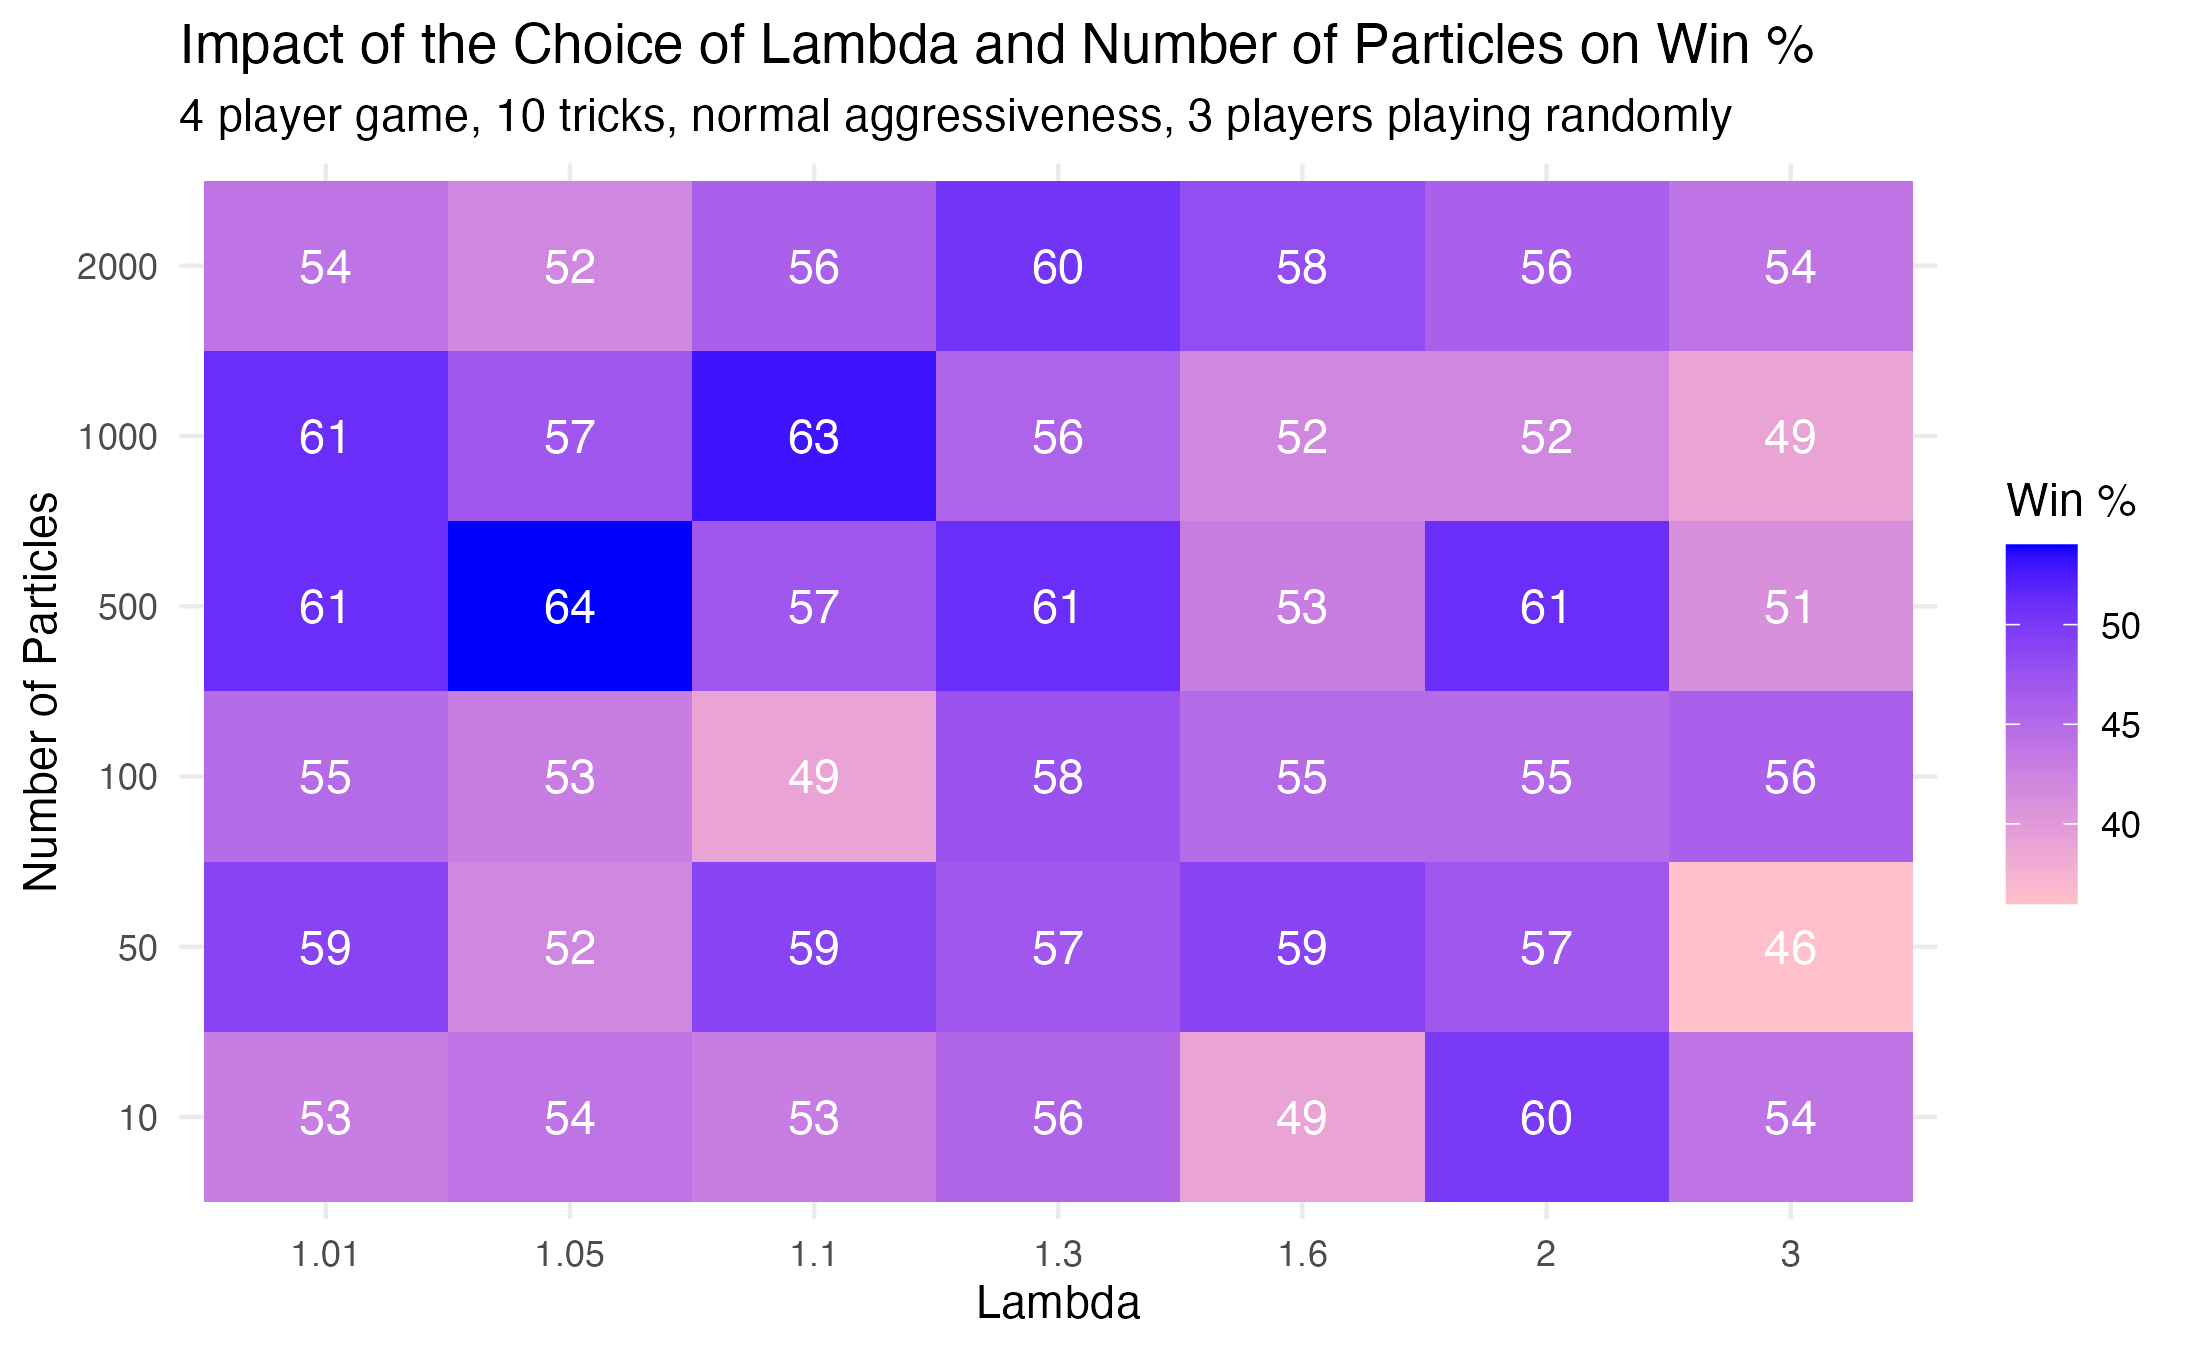
\includegraphics[width=\linewidth]{lambdavsparticles.png}
\caption{Comparing performance of AI player for different number of particles and value of $\lambda$}
\label{fig:partslambda}
\end{figure}

Next, in order to confirm the validity of our bidding algorithm, we have our AI player play against 3, 2, and 1 random player(s), and try 3 different bidding modes: passive, normal, and aggressive. The "normal" mode just uses whatever our bidding algorithm spits out. The passive mode reduces the predicted bid by one, and the aggressive mode increments the bid by one. In theory, if our bidding algorithm is performing well, the AI player should have the highest winning percentages using the "normal" bidding approach. 

Figure~\ref{fig:mcagg} displays the results for each number of players and each number of tricks. These results indeed show that our bidding algorithm is working. It is interesting to note the extent to which the normal bidding strategy out performs the other two. In a 4 player game, since there are more players competing for tricks, it is harder to win an extra trick. This is why the aggressive mode performs so poorly. On the flip side, when there are more tricks available to win, it becomes easier to win different number of tricks as there is more time for the player to adjust their strategy. Both of these trends can be seen in each of the plots in Figure~\ref{fig:mcagg}.
\begin{figure}[H]
  \centering
  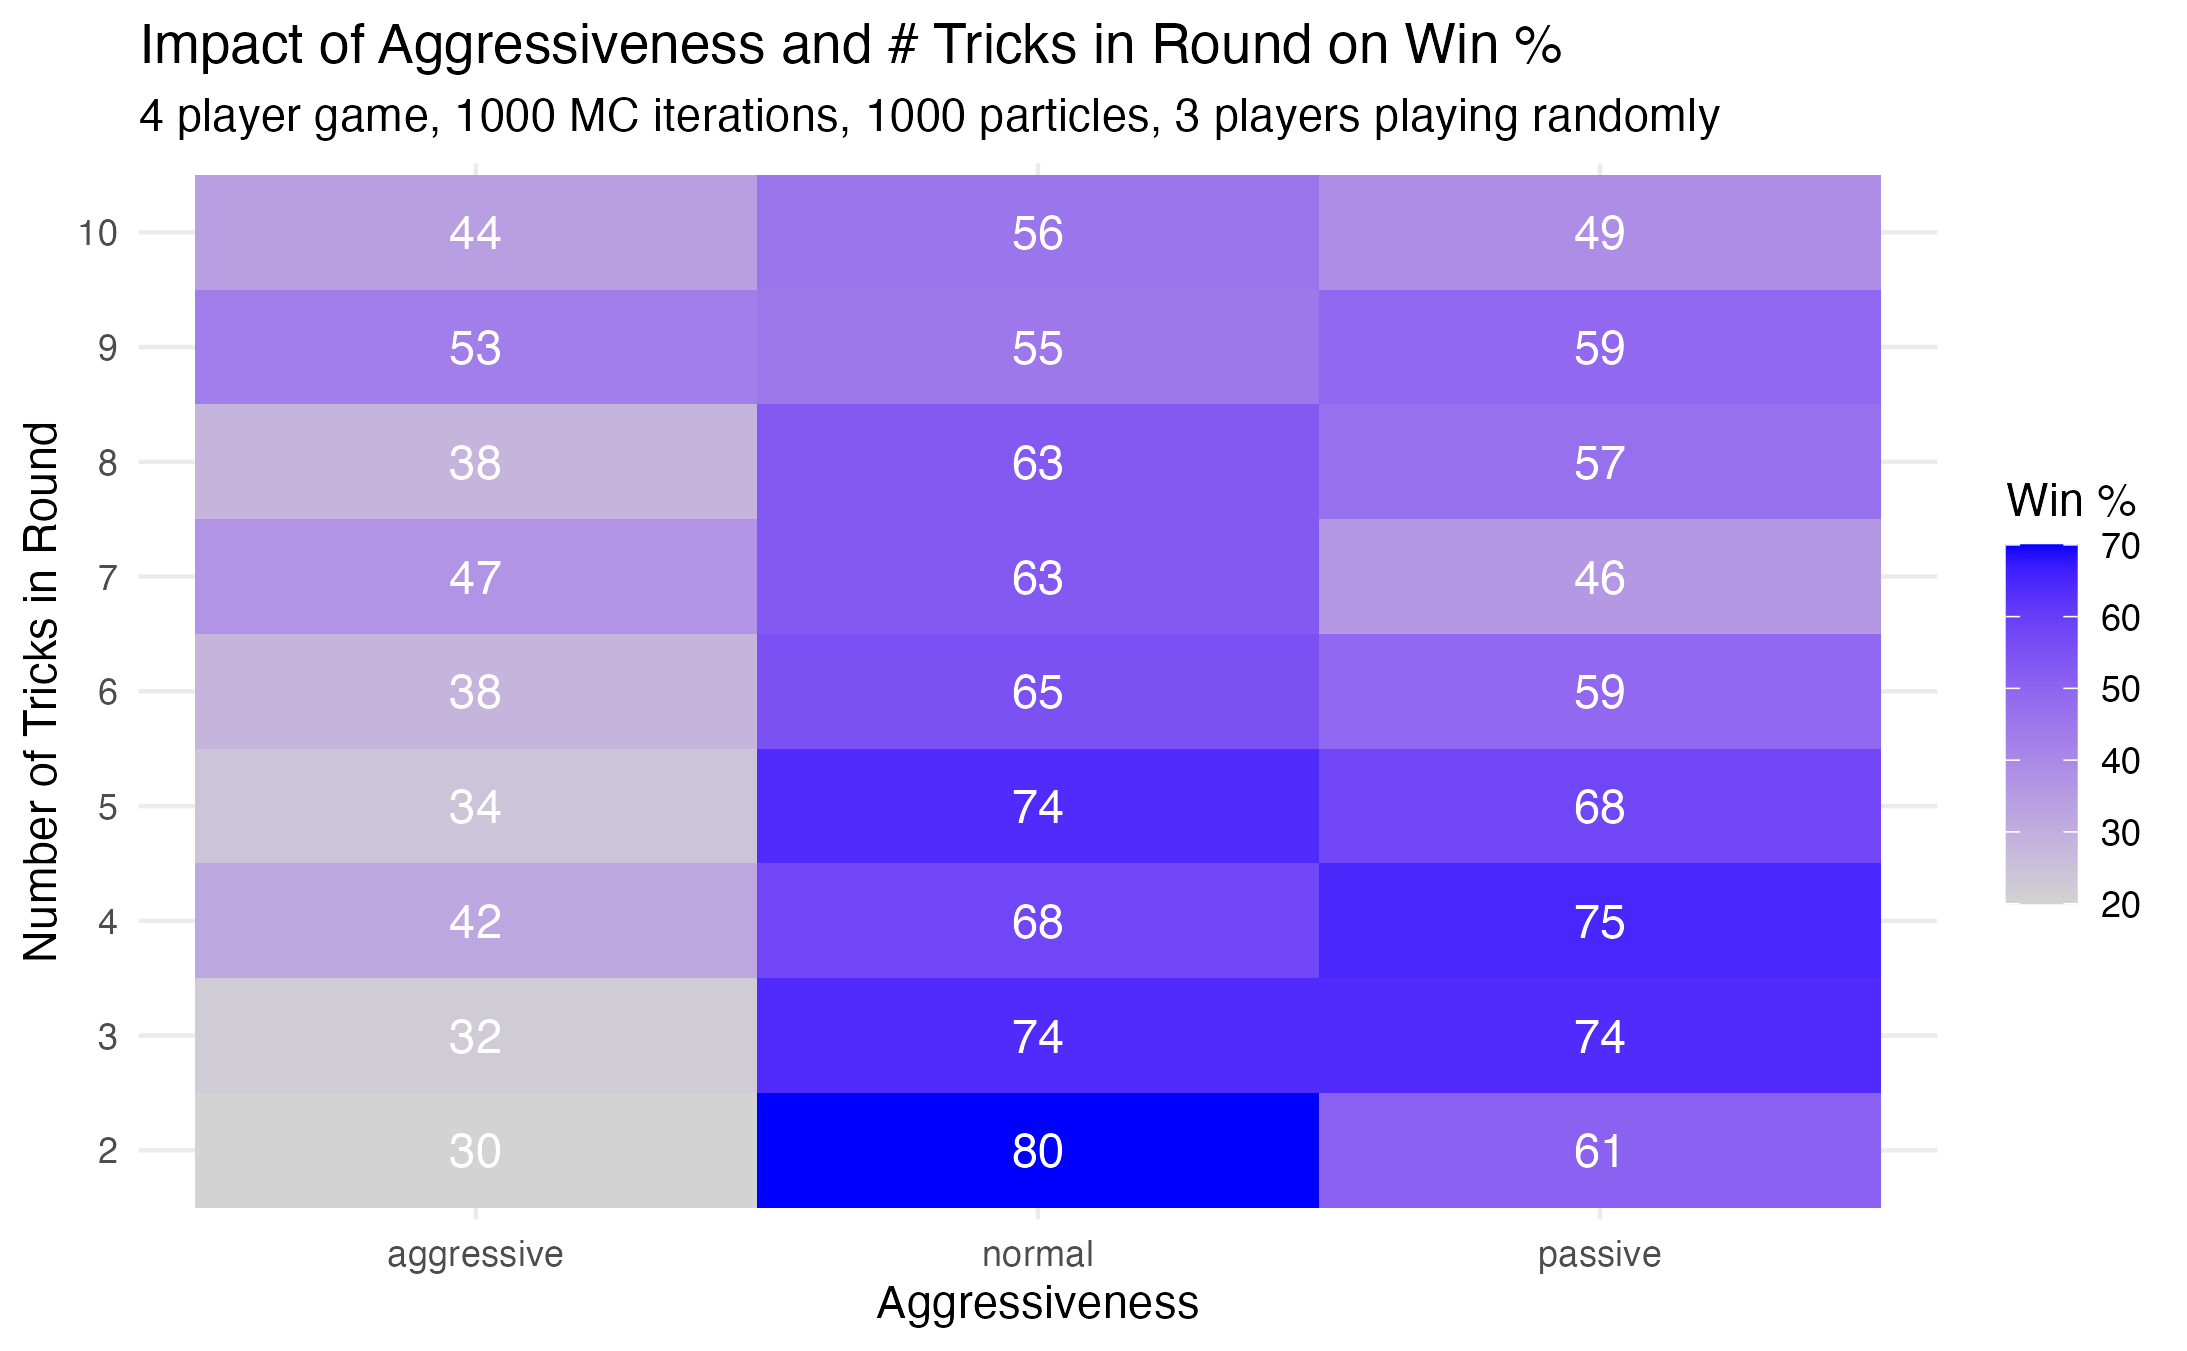
\includegraphics[scale=0.55]{mcvsagg4.png}

  \medskip

  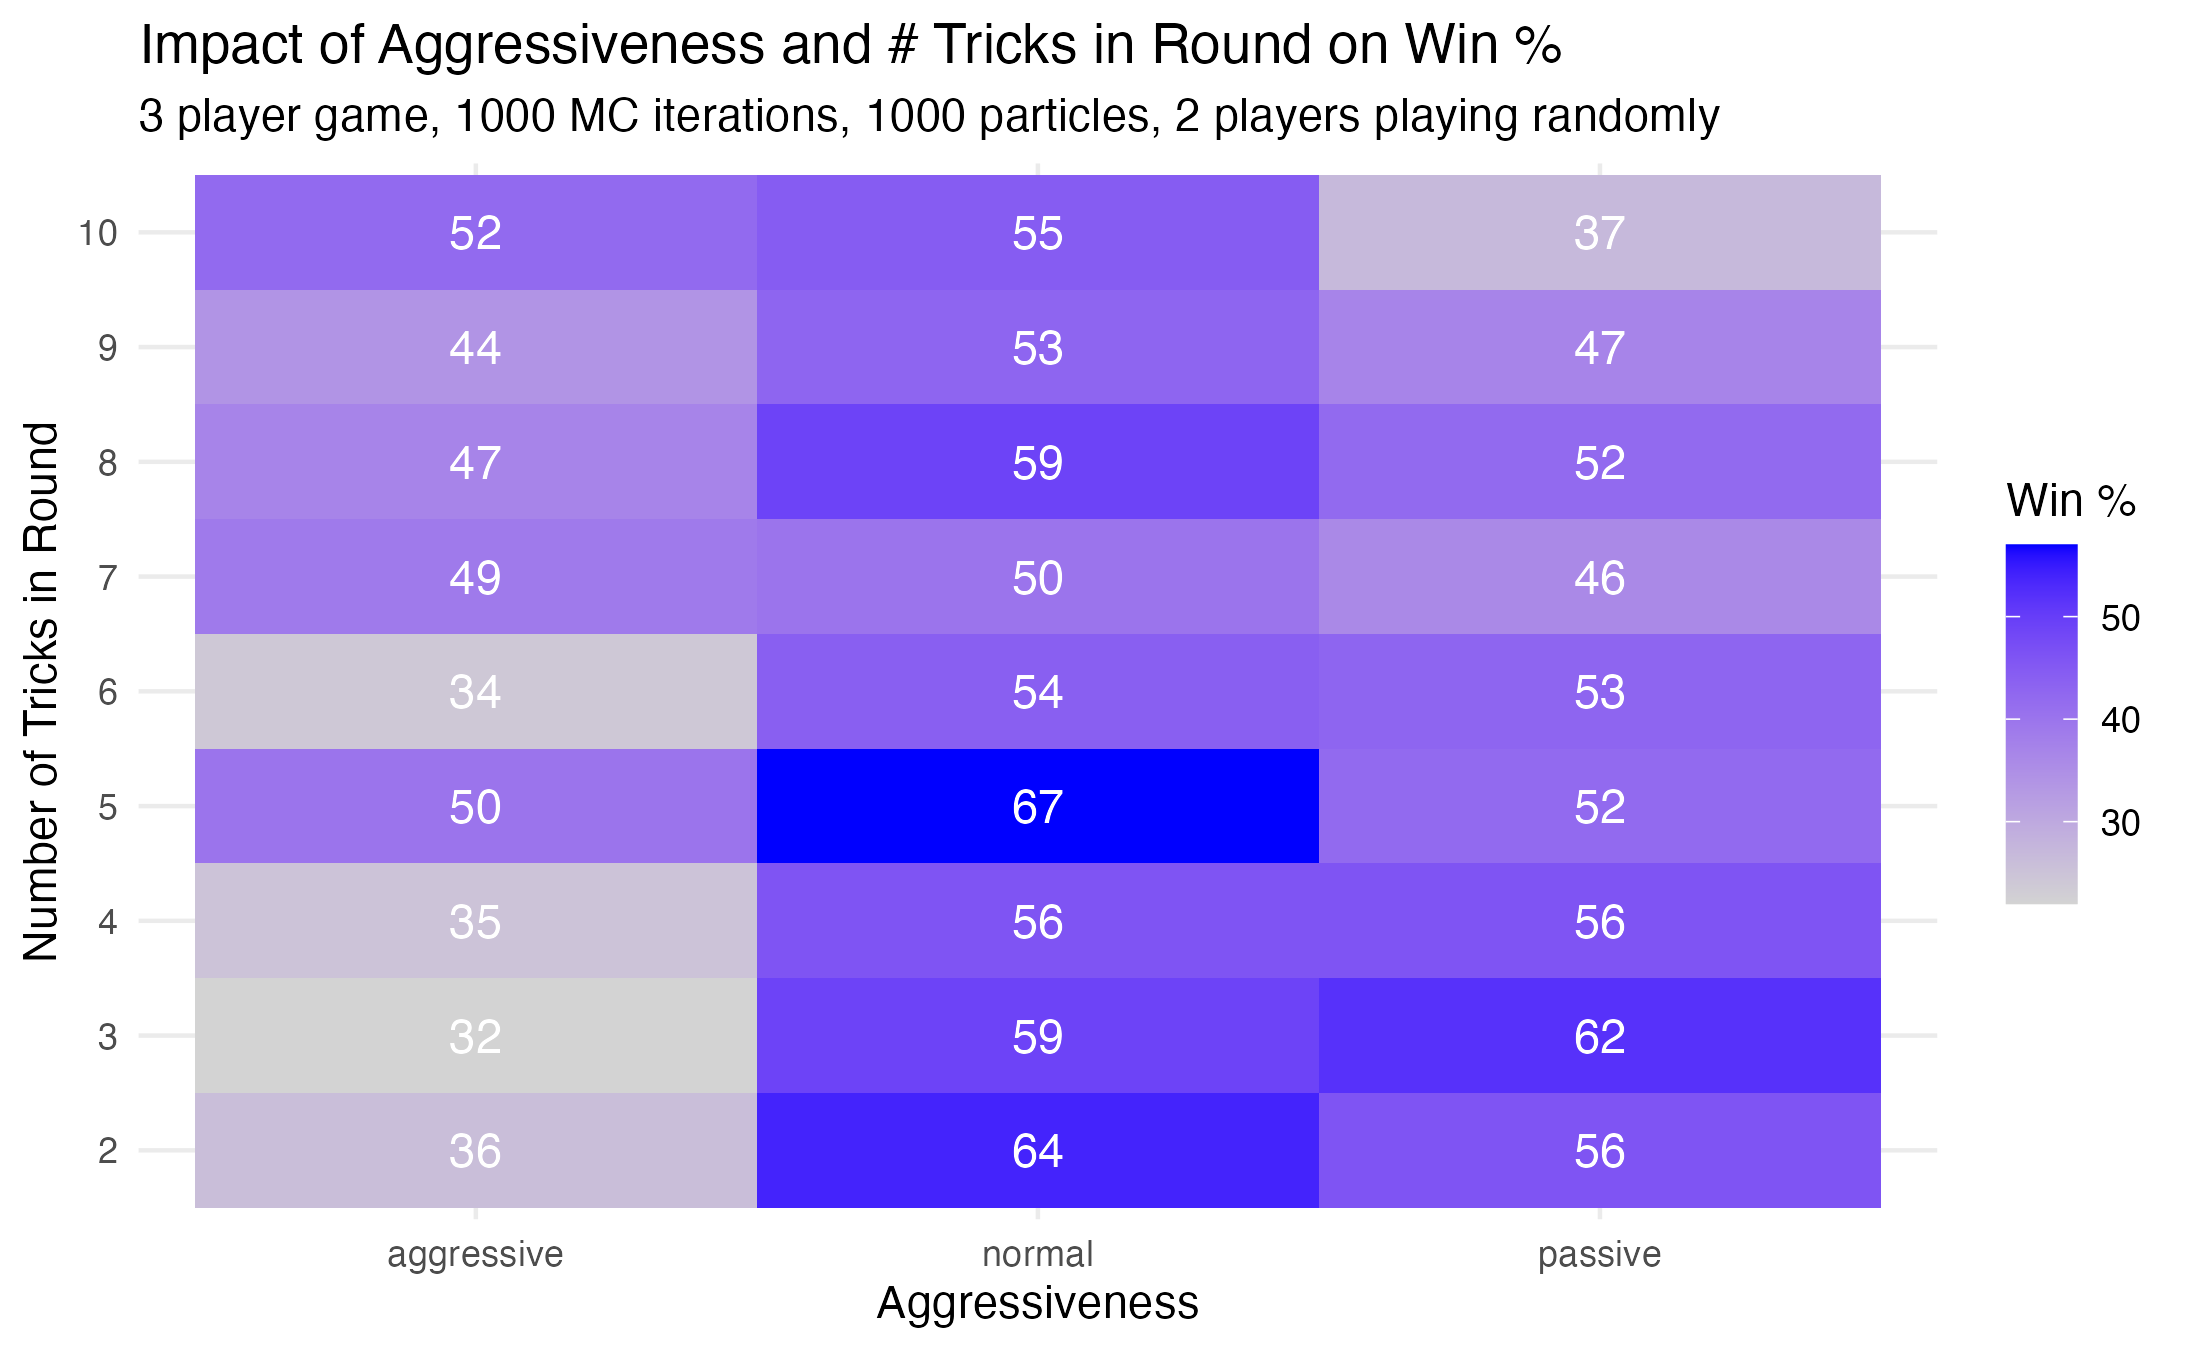
\includegraphics[scale=0.55]{mcvsagg3.png}

  \medskip

  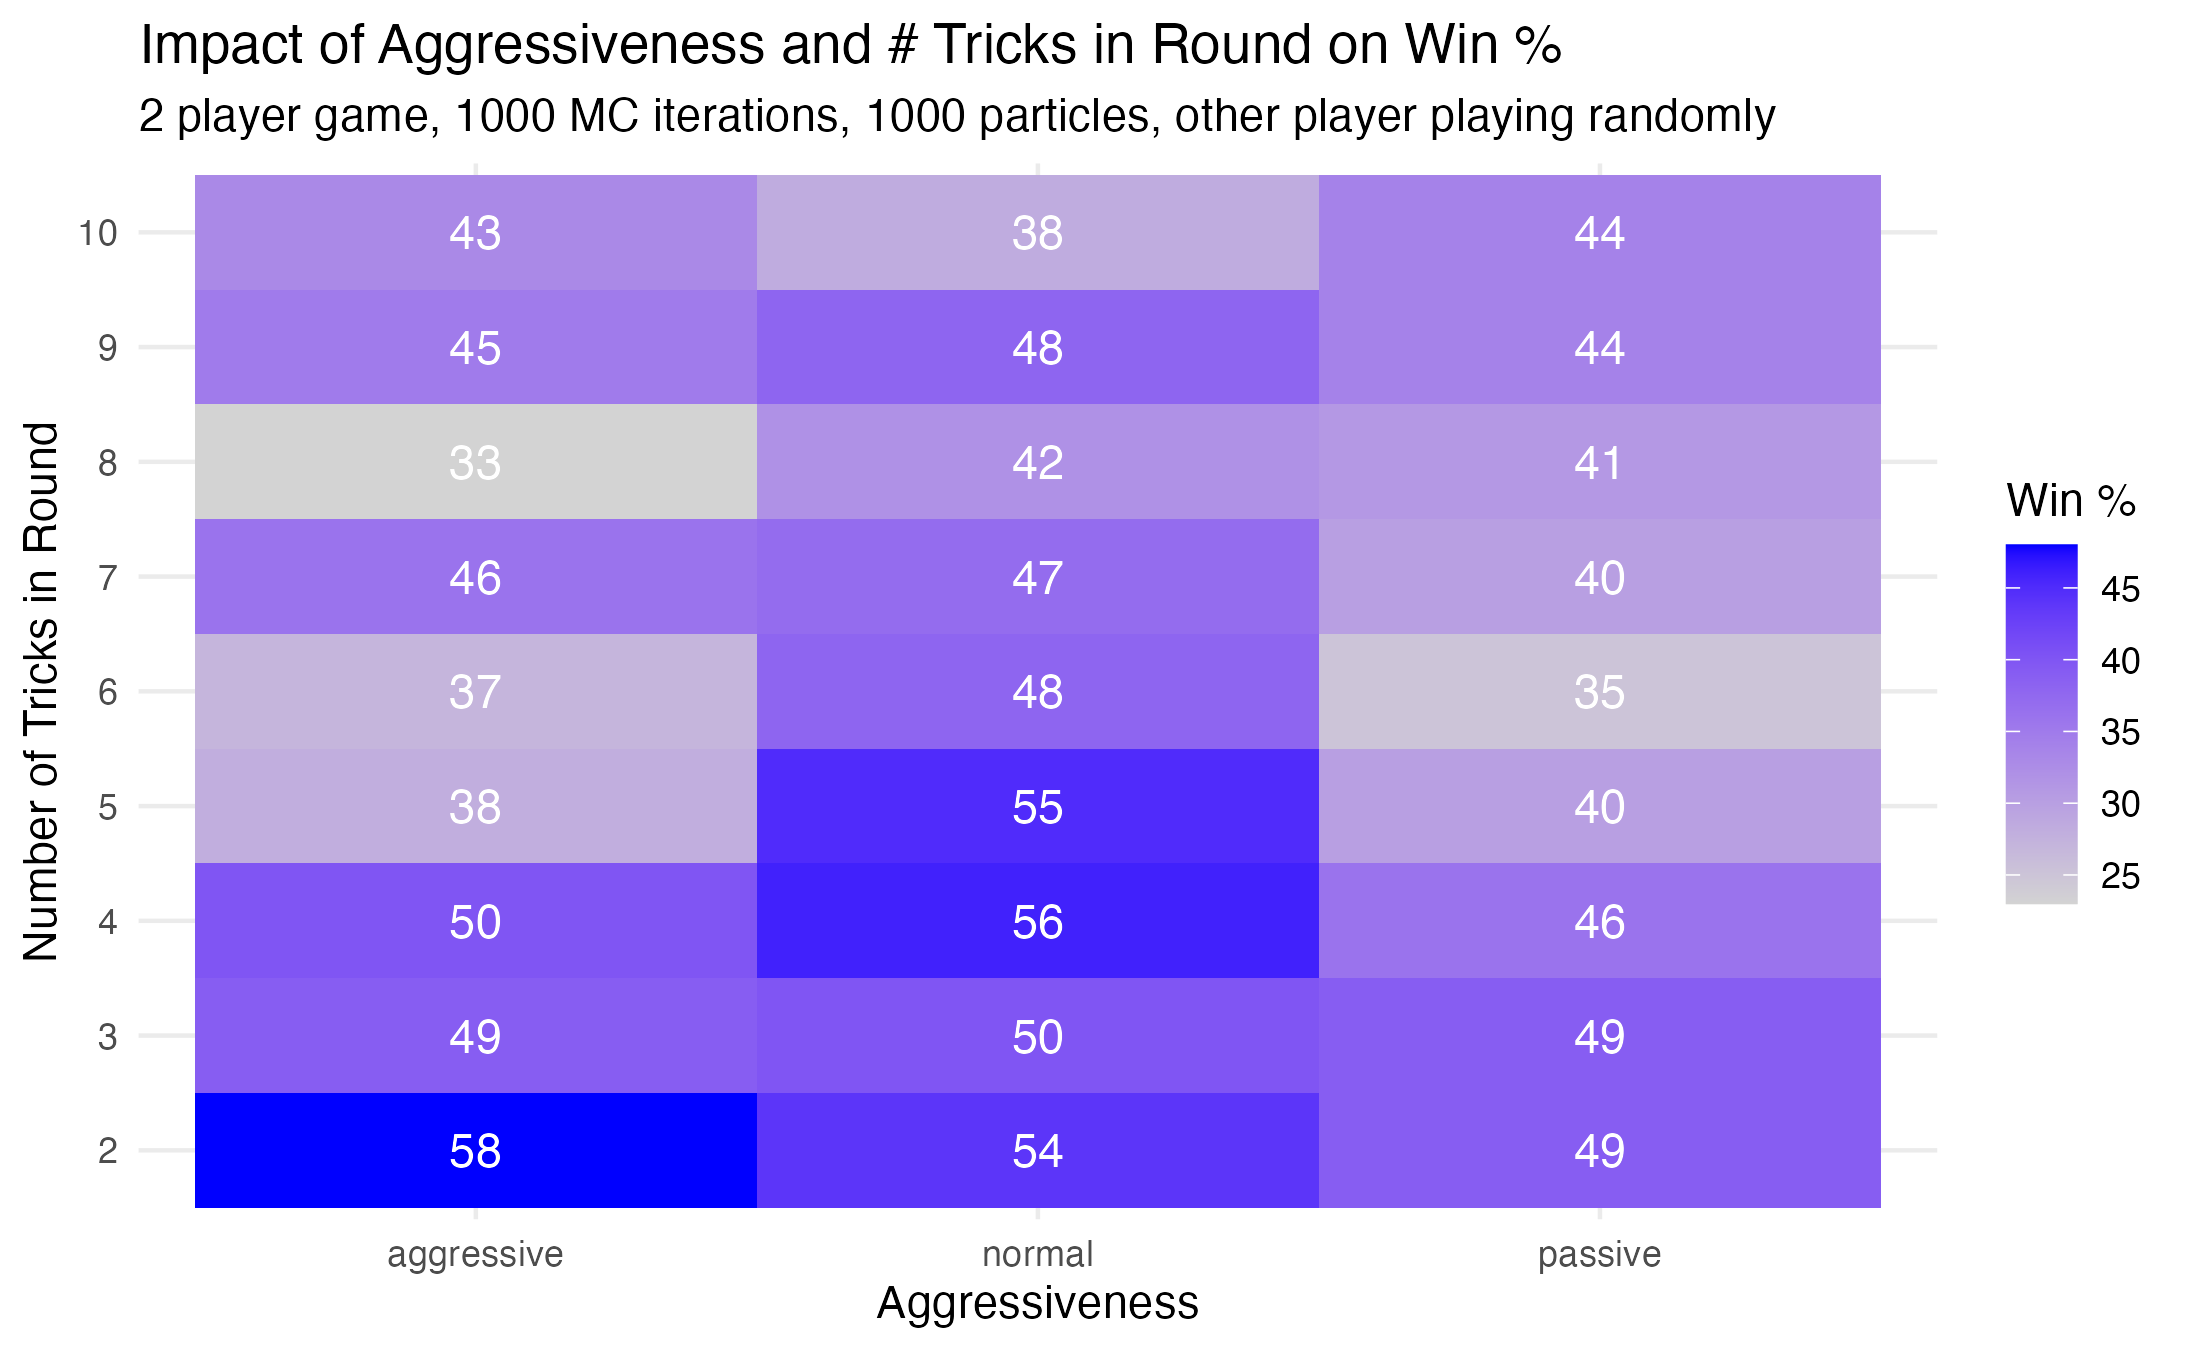
\includegraphics[scale=0.55]{mcvsagg2.png}

  \caption{Comparing performance of AI player against randomly playing players across different numbers of tricks and bid aggressiveness}
    \label{fig:mcagg}
\end{figure}

\leavevmode\\
In our final experiment to assess the AI's aptitude, we simulate thousands of 4 player games where all players are using our AI model. The first player uses 1 iteration of ISMCTS, the next uses 10, then 100, then 1000 for player 4. We'd expect that player 4 would do the best as they have the strongest playing model. Indeed, looking at Figure~\ref{fig:mctricks}, we see that the win percentages generally increase as we go left to right. Note that win percentages are lower across the board with 9 and 10 trick rounds, as with lots of tricks there is more variance which makes it harder to win. Player 3 and Player 4 are quite comparable overall, with Player 4 having a slight edge. This may indicate that 1000 simulations isn't necessary to achieve good performance.
\begin{figure}[H]
\centering
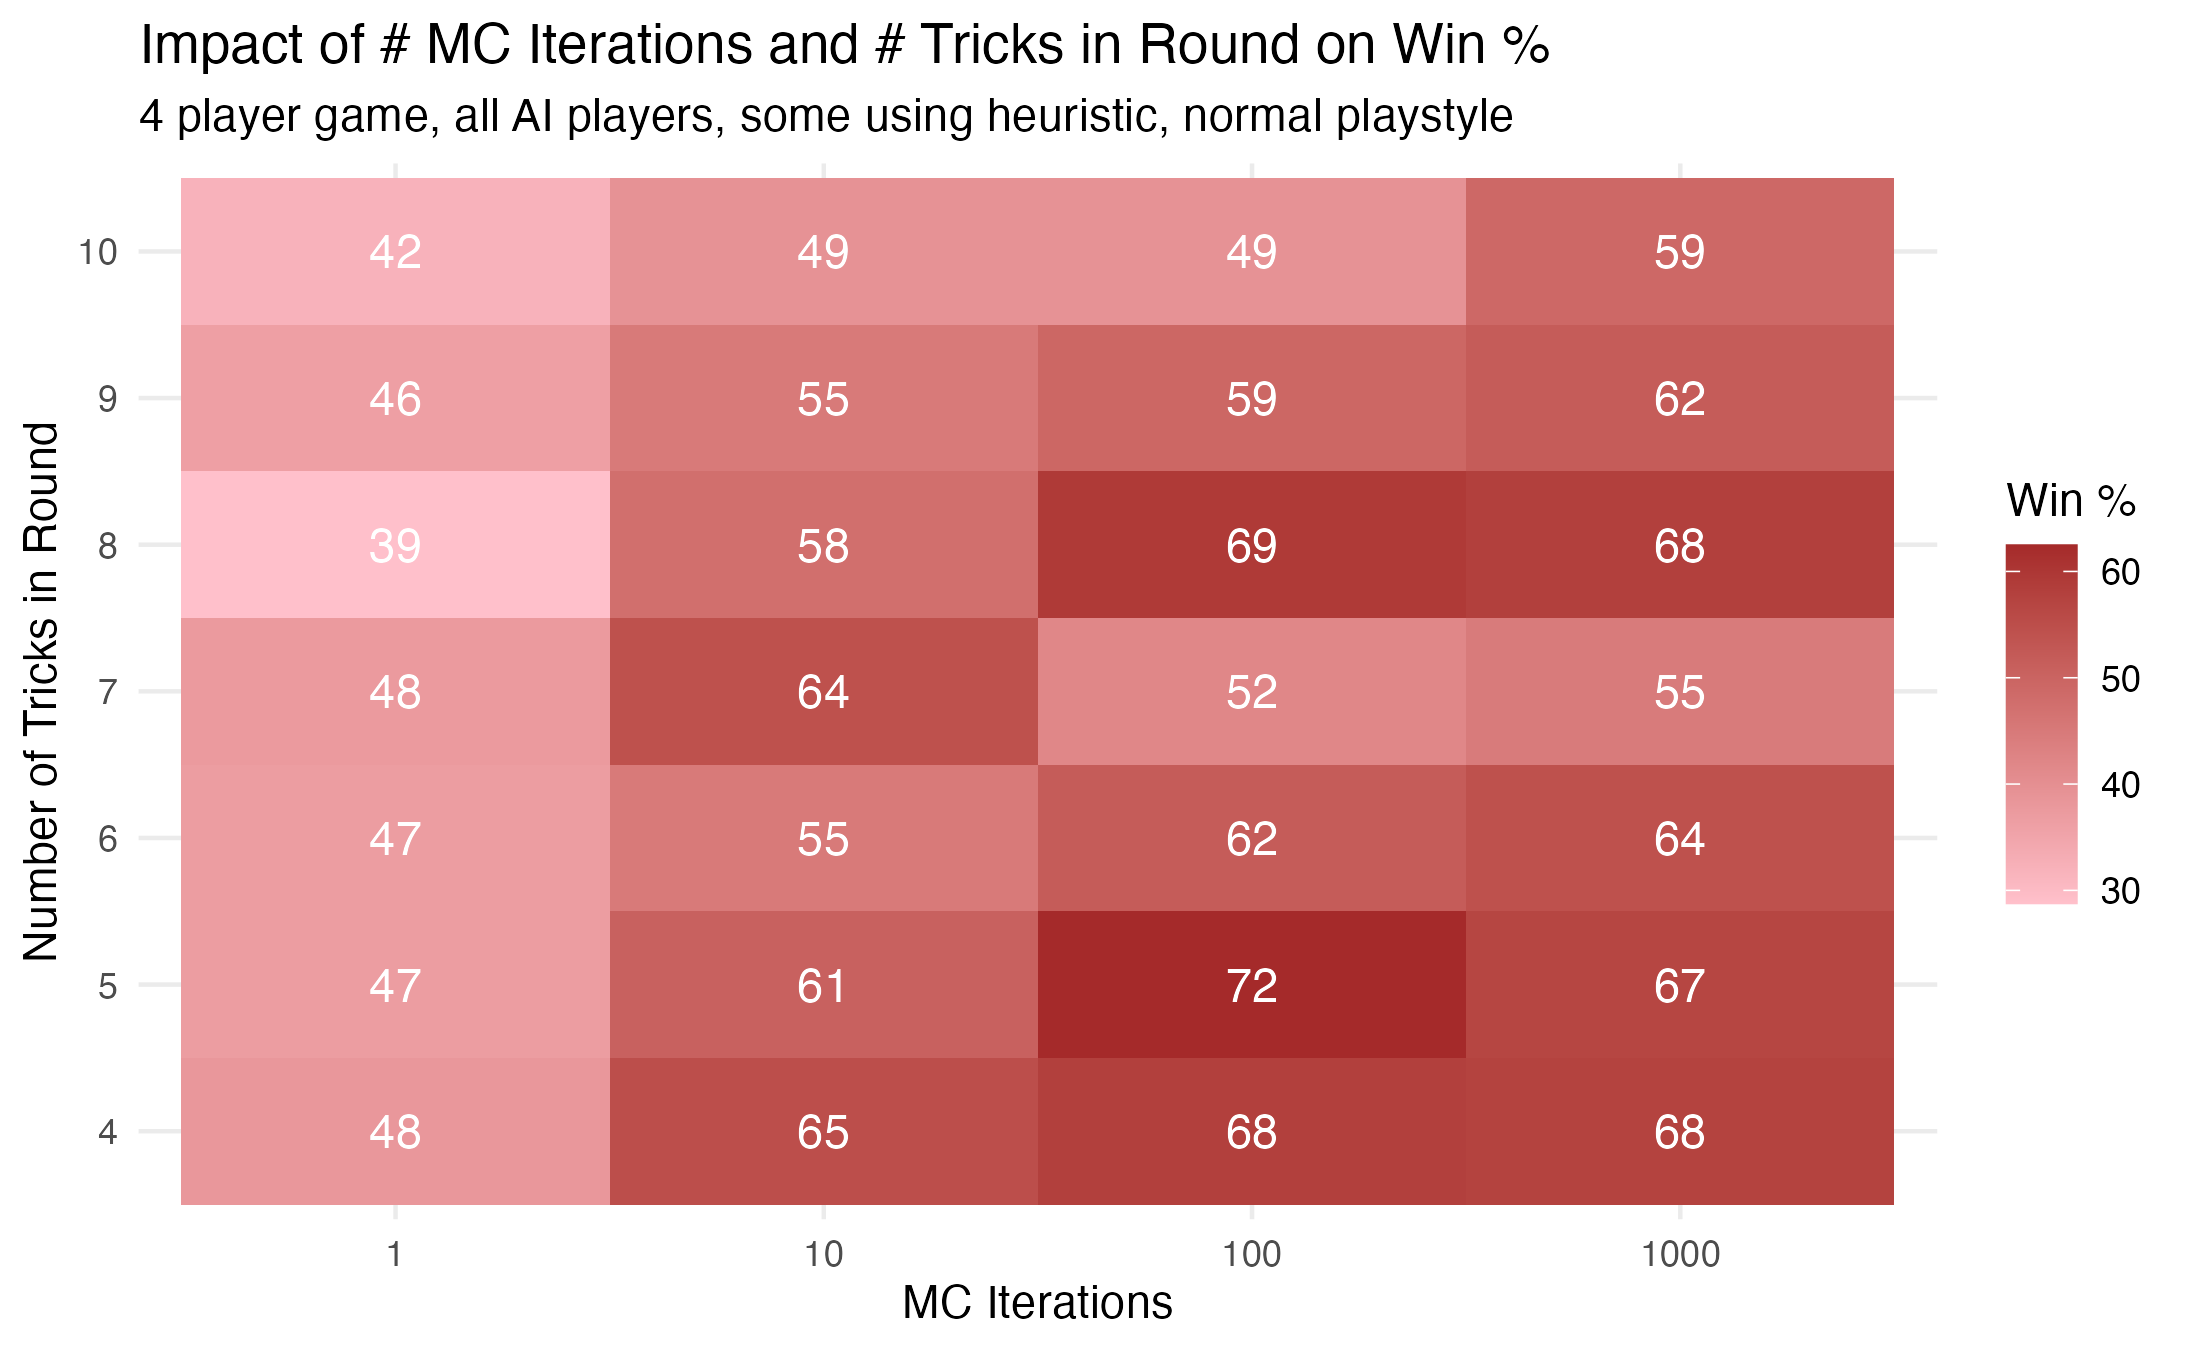
\includegraphics[width=\linewidth]{mcvstricks.png}
\caption{Comparing performance of AI players for different numbers of tricks and different numbers of ISMCTS iterations. Player 1 ran 1 sim, Player 2 ran 10, Player 3 ran 100, Player 4 ran 1000}
\label{fig:mctricks}
\end{figure}

Finally, how does the AI actually play? To test this, we wanted to see what type of card is typically played by the AI when it has the lead (meaning it plays first in a trick and can play any card). We hypothesized that the card they play should be directly linked to the number of tricks that they win. While this is a bit of an oversimplification as there are many other factors that are not captured, it is a good baseline to see the general strategy of the AI. 
Figure~\ref{fig:playstyle} displays the results. 

Data for times when the AI needed to win more than 5 tricks or less than 0 tricks (i.e. they've won 2 more tricks than they bid) were omitted due to a small number of occurrences. We can see that, when needing to win multiple tricks, the AI favors playing a high (Jack or Queen) or very high (King or Ace) off suit card. 
This is a solid strategy as, to win a trick with an off suit high card (one of three ways we can win a trick), it is made a lot easier when you are able to lead that card, and lead it early, to try and mitigate the possibility of other players trumping in. The AI player favored playing a low off suit card when it didn't need to win any more tricks, playing such a card (2-6) $43\%$ of the time. 
It is interesting to note the lack of trump cards that are lead. This makes sense given it is advantageous to hold onto trumps in the hopes of trumping in, and, in conjunction, lead an off suit to try and lose all cards of that suit. The highest played trump scenario was when the AI needed to win 0 tricks and played a low trump. 
This likely occurs towards the end of a game when the AI knows that other players need to win tricks, so it trusts that it can lead a low trump and someone else will play a higher one and take the trick. Overall, this data makes sense with conventional human thinking around what to play when leading.
\begin{figure}[H]
\centering
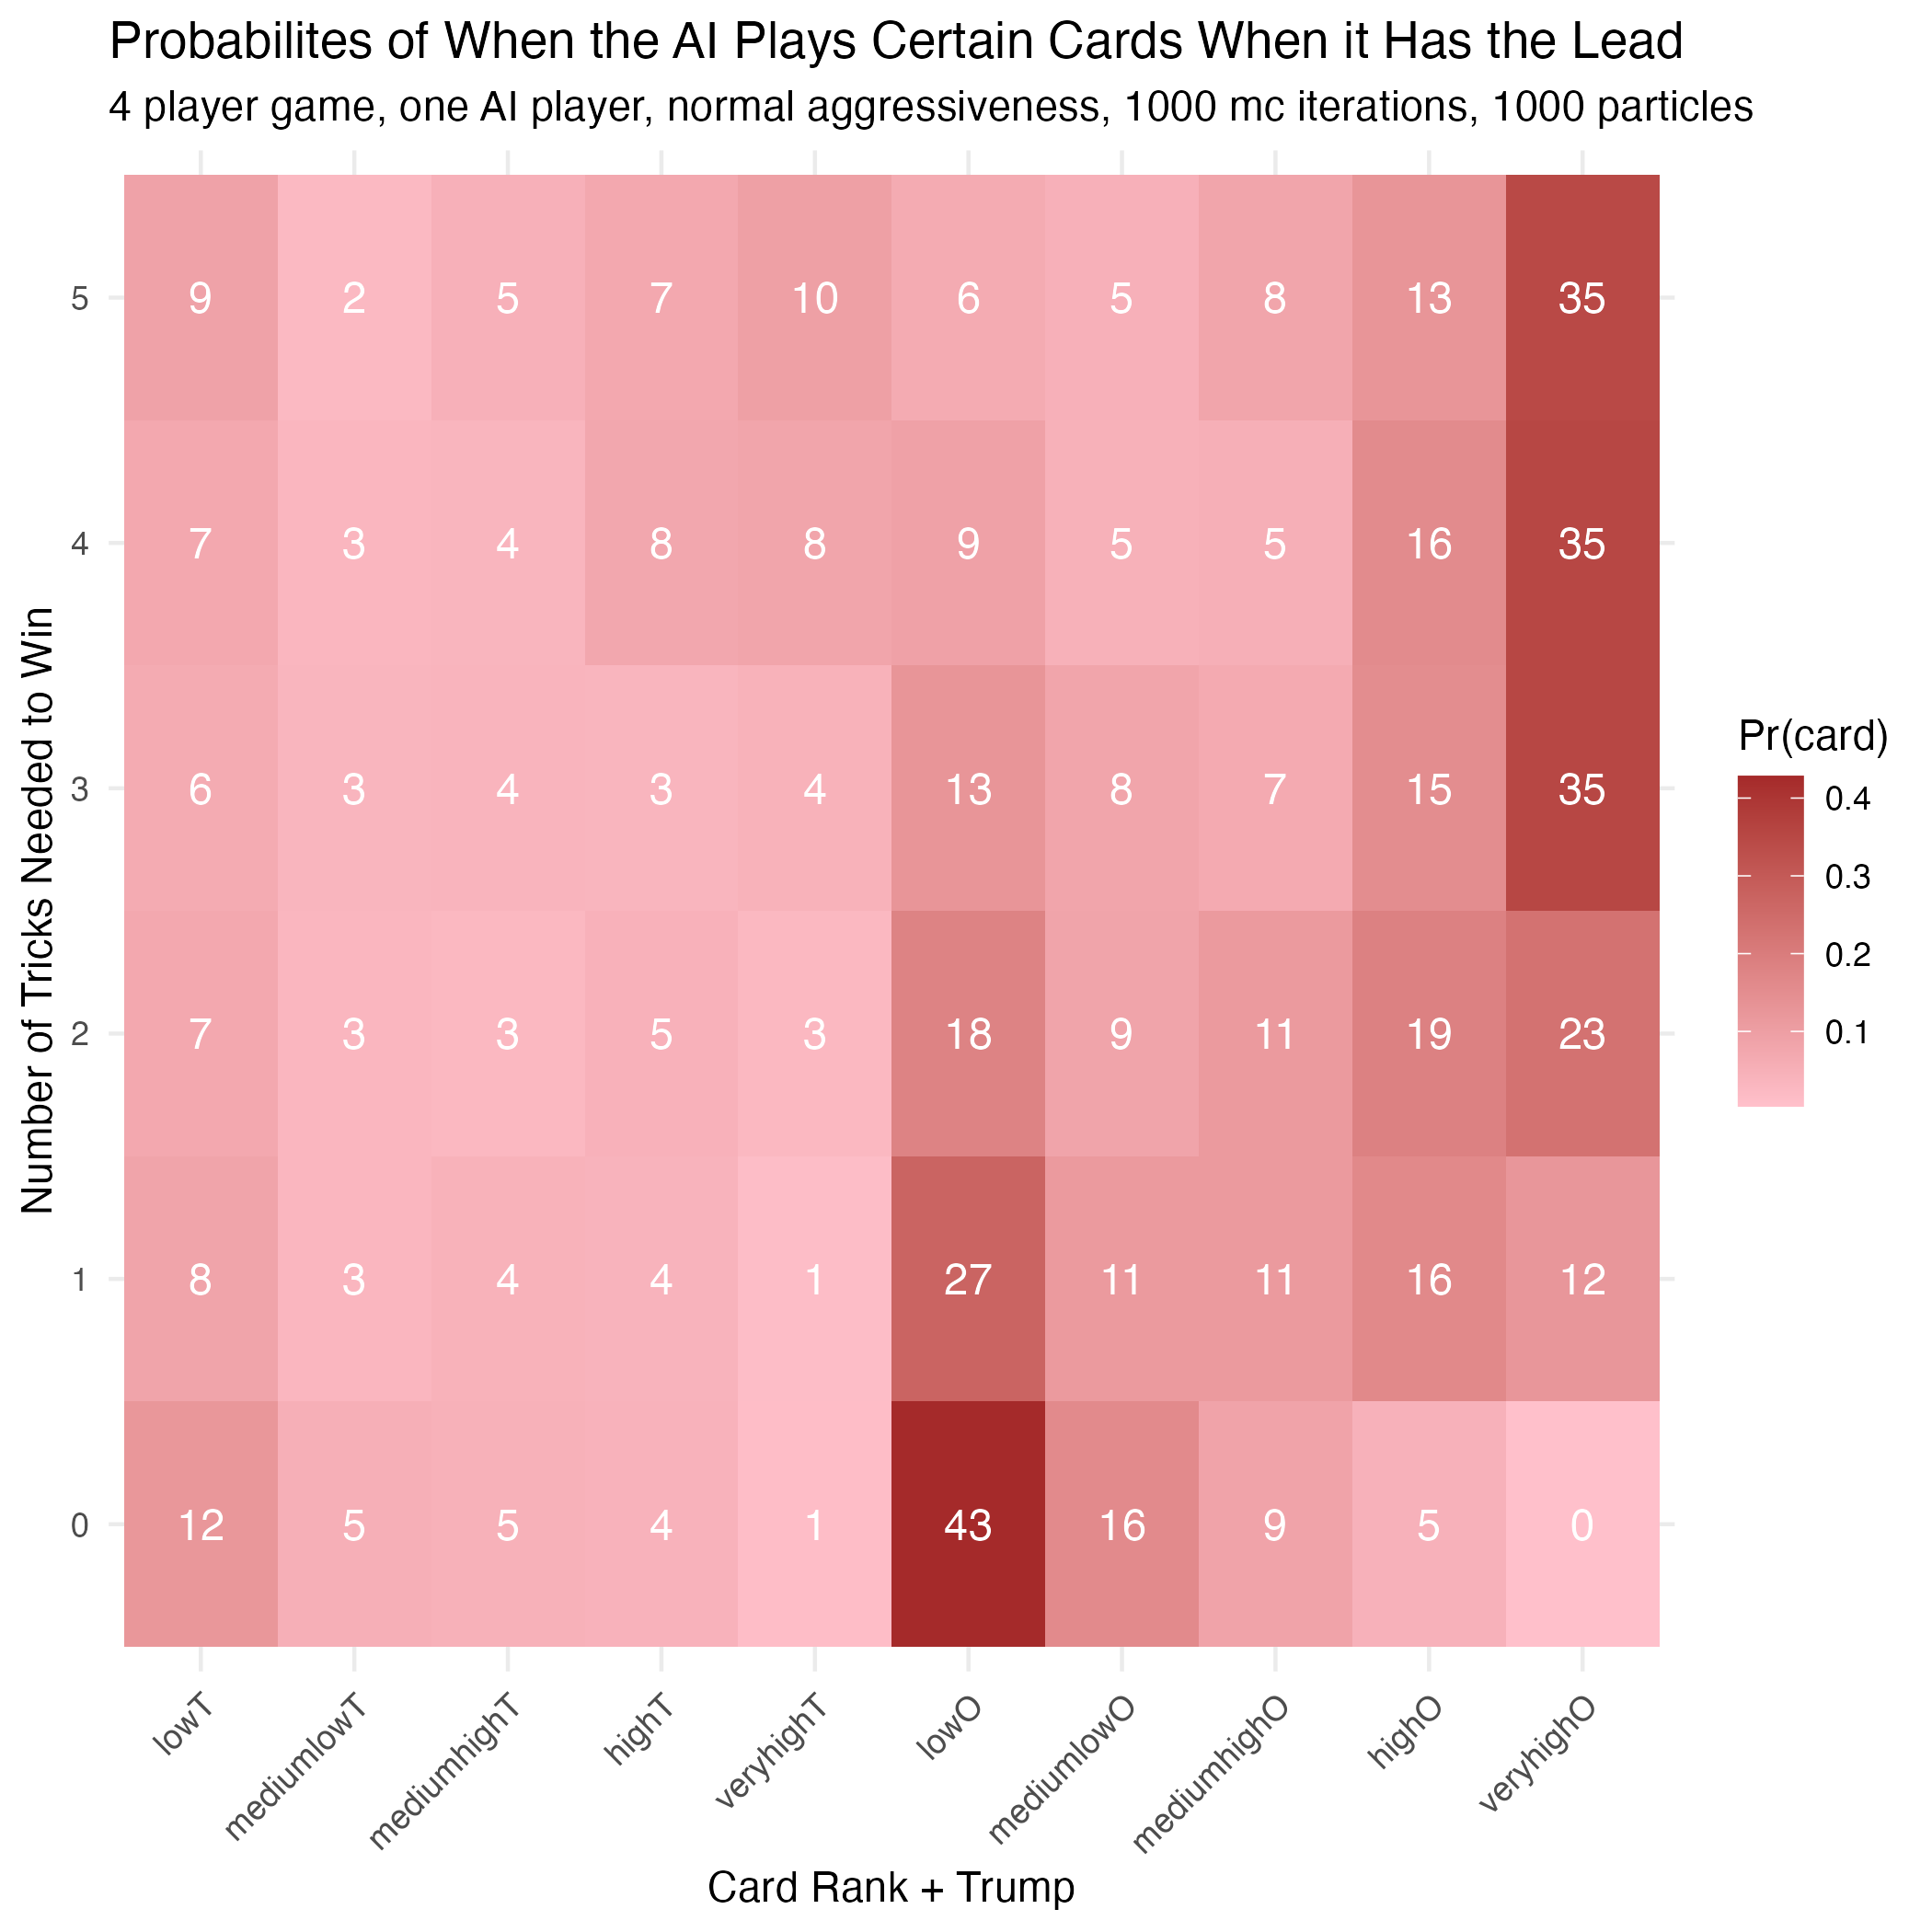
\includegraphics[width=\linewidth]{playstyle.png}
\caption{Probabilities of the AI player leading a certain card of suit trump/offsuit depending on how many tricks it needs to win. Low rank (2-6), mediumlow (7-8), mediumhigh (9-10), high (Jack or Queen), veryhigh (King or Ace)}
\label{fig:playstyle}
\end{figure}

\section{Future Work}
\label{section:FutureWork}
While our AI player seems to perform quite well, there are still tests to be done to tune parameters and dive deeper into how it plays. This might help us discover edge cases where the AI does not play optimally. To help it play better, more heuristics can be added during the determinization phase of ISMCTS. While this does reduce the speed of the algorithm, it will improve its play and make it more human-like if it's using common strategies. The beauty of ISMCTS, though, is that those strategies need not be hard-coded into the bot and it can learn the best way to play.

Additionally, creating a more user-friendly interface for a human to play against the AI would make it easier and more palatable to potentially develop an online version of Oh Hell that would use this AI player. Right now, everything is run and shown in the output window via text, which isn't as visually appealing. Finally, the best way to discover deficiencies in our AI player is by playing against it. This takes time, but might help to uncover any exploitable moves the AI consistently makes.


\section{Conclusion}
\label{section:Conclusion}
In this paper, we demonstrated the playing capabilities of our AI to play the card game Oh Hell. We developed our own bidding algorithm that incorporates the player's hand, the position in which they bid, and the total number of bids prior to them. Then, our AI uses Information Set Monte Carlo Tree Search to find the best move when it is their turn given the state of the game. We discuss how our AI determinizes the given state through the use of particle filtering. Employing heuristics and sampling techniques, the AI builds a probability distribution of the possible hands that its opponents have at any given point in the game. Then, we analyze the performance of the AI player by running simulated games and discussing what parameters influence its strength, as well as the strategies the AI uses to try and win each round. 
These experiments show that our AI player is a strong Oh Hell player and is fit to play at a comparable level to a strong human player.

\bibliographystyle{unsrtnat}
\bibliography{sample}

\end{document}
